 % -*- encoding: UTF8 -*-
%
%%*****************************************************************************
%%												Design & Simulation										                                        
%%*****************************************************************************

\chapter{Design \& Simulation}
\label{Ch:DesignSimulation}	

The aim of this work is to design and test a miniaturized OCT microscope as a component of a multi-modal endoscope. As described in Chapter \ref{Ch:Introduction}, this probe consist of two spectrally-separated optical paths that run partially in parallel through a micro-optical bench system. This approach allows independent tuning of the optical parameters of the two imaging modalities -- such as the NA or depth of field -- while still providing a geometrical overlap of the two acquired images. An integrated tubular piezoelectric fiber scanner is used to perform en face scanning required for three dimensional OCT measurements. This scanning engine has an outer diameter of 0.9 mm and a length of 9 mm, and features custom fabricated \SI{10}{\micro\meter} thick polyimide flexible interconnect lines to address the four piezoelectric electrodes.

The following section describes the conception and design of the endoscope, starting from the medical and geometrical requirements, through analytical modeling and towards the optimization of each component.

%%*****************************************************************************
\section{Design Requirements}
%%*****************************************************************************



The OCT microscope should fulfill the following requirements:

\paragraph{Mechanical Requirements} 
\begin{itemize}

\item The scanner, electrical connections and optics should fit in a $\SI{1}{\milli\meter} \times \SI{1}{\milli\meter}$ square channel. Its length should be minimized.
\item The field of view should be maximized for a 2 mm diameter objective lens.
\item The scanning speed should be adequate for the sampling rates characteristic of OCT ($\sim \SI{100}{\kilo\hertz} $).
\end{itemize}


\paragraph{Optical Requirements}

\begin{itemize}
\item The microscopy and OCT imaging fields should be coaxial to avoid parallax errors. 
\item The OCT field should be image-side telecentric to avoid field curvature distortions and to maximize the collection of backscattered light upon normal incidence to the tissue.
\item The lateral resolution and depth of field should be adequate for OCT (Numerical aperture 0.02 to 0.05).
\item The backreflections inside the probe should be minimized.
\end{itemize}

  

%%*****************************************************************************
\section{Design overview}
%%*****************************************************************************

The main challenge of this work is to design a scanning mechanism compact enough to be placed in a thin, buried channel of a multimodal probe. 
Although it is theoretically possible to keep a scanner at the proximal end of the endoscope and use a coherent fiber bundle (CFB) as a relay, there are inherent drawbacks of this method, such as low light throughput, cross-talk and mechanical rigidity \cite{Ford2009}. 

Another challenging requirement is the superposition of the images acquired by the different modalities. If the optical axes are not coaxial, the fields will be shifted and tilted due to parallax error --- which gains importance at the small working distances common in endoscopy.

To overcome these problems, and taking into account the above-mentioned requirements, we propose a design comprising a resonant fiber scanner followed by a beam splitter, as illustrated in Figure \ref{fig:bimodalSketch}, as an evolution of the HYAZINT multimodal probe \cite{Kretschmer}.

\begin{figure}[h!]\centering
      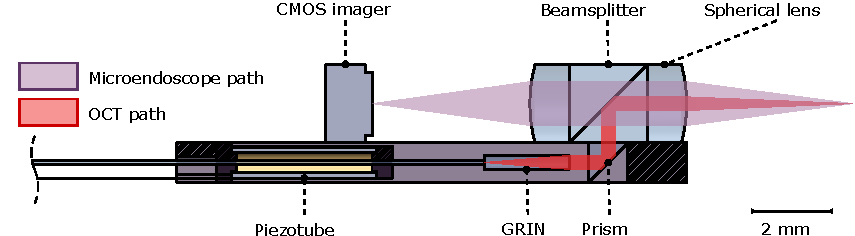
\includegraphics{figures/10_Introduction/bimodalSketch/out.pdf}
      \caption{Bimodal probe cross section showing main components and optical paths.}
      \label{fig:bimodalSketch}
\end{figure}

This implementation uses a piezo tube actuator which drives a bending beam into a resonant oscillation. This bending beam is composed of an optical fiber with a GRIN lens glued to its tip which, due to the oscillation of the fiber, scans radially a collimated laser beam. An objective lens then transforms this angular displacement into translation, as explained in Chapter \ref{Ch:Theory}. In order to merge the OCT field with the white light image, both fields are combined using a dichroic beam splitter.

There are many reasons why this design is preferred over other scanning topologies. First, the narrow dimensions of the piezo tube allow a compact implementation. Also, the field of view that can be achieved with this scanner is not limited to the space available for the GRIN lens to vibrate --- instead, to its maximum angular deflection. As we want a telecentric system, a \textit{4f} microscope could have been implemented instead of a Fourier plane scanner, but at the cost of duplicating the length of the optical system (Chapter \ref{Ch:Theory}). Another advantage of using a fourier plane scanner is that it requires a GRIN lens glued to the tip of the fiber in order to collimate the beam. As a side-effect, this extra weight greatly reduces the resonant frequency of the scanner, allowing a denser sampling from the data acquisition system. 

The rest of this chapter shows the design and development of the OCT imaging path for the multi-modal probe. However, in order to independently test the behavior of the OCT scanner and optics, a single modality probe was fabricated as a demonstrator. Both systems are mechanically and optically equivalent -- the only difference is the presence of the beam splitter. 

For completeness, both multi-mode and single-mode optical systems are described.


%%*****************************************************************************
\newpage
\subsection{Optical Design}
%%*****************************************************************************

\subsubsection*{Fourier Plane Scanner}
The OCT beam path is designed as an object-sided telecentric system to avoid distortions in the 3D OCT measurement. To achieve this, the fiber scanner is driven with small angles and is positioned such that the lateral and angular movement of the scanner imitates the beam angles that can be observed in the collimated region of a classical telecentric lens system. Figure \ref{fig:fps} illustrates this approach. The whole scanner will be buried in a channel with a inner diameter of \SI{1}{\milli\meter} limiting the movement of the scanner to a maximum angle $\theta$ of \SI{5}{\degree} that allows a maximum FOV of \SI{1}{\milli\meter} of the OCT beam path.



\begin{figure}[h!]\centering 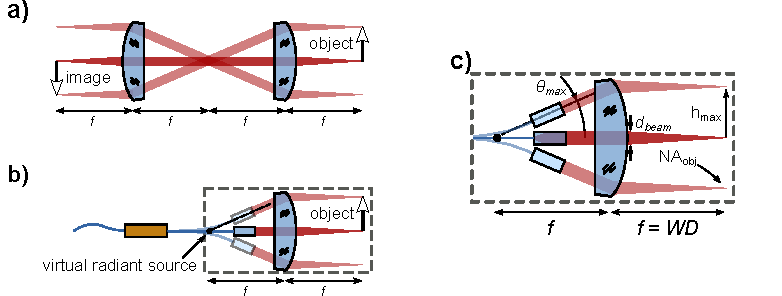
\includegraphics[width=\columnwidth]{figures/30_DesignSimulation/fps.pdf}
      \caption{\textbf{a)} Illustration of a classical telecentric system. The height of the object is translated into an angle $\theta$ in the collimated region between the two lenses. This angle is again translated into a corresponding image height by the second lens. \textbf{b)} Illustration of the OCT beam path using a fiber scanner in first resonance mode without micro prism and BS. The movement of the GRIN lens due to the fiber scanner and the distance between the GRIN lens and the focusing lens creating the same optical behavior as it can be observed in a classical object sided telecentric system. \textbf{c)} Close-up showing the design variables.}
      \label{fig:fps}
\end{figure}

\subsubsection*{Component Selection}

In a Fourier plane scanner, the numerical apertures (NAs) and focal lengths of the scanning (GRIN) and objective lens are interdependent by the diameter of the beam in the intermediate region. Thus, following the schematic of Figure \ref{fig:fps}c, we can obtain the following relationships by geometrical optics\footnote{For small NAs: $\tan[	\sin^{-1}(\mathit{NA})] \simeq \mathit{NA} $. For example, if NA = 0.2, the error of this simplification is 2\%. }
\begin{align}
d_{beam} &\simeq 2\cdot \mathit{f_{GRIN}}\cdot \mathit{NA_{fiber}} \\
d_{beam} &\simeq 2 \cdot f_{obj}\cdot \mathit{NA_{OCT}}
\label{eq:fpsNA}
\end{align}

By combining them together we arrive to the main design equation for the scanner:
\begin{equation}
\mathit{f_{GRIN}} \cdot \mathit{NA_{fiber}} = f_{obj} \cdot \mathit{NA_{OCT}}
\end{equation}

The design of the optical path for OCT is constrained by the commercially available components. In this case, the only single mode fiber working in our wavelength range and with thinned cladding diameter (\SI{80}{\micro\meter}) is \textit{Thorlabs SM980G80}, with $\mathit{NA_{fiber}} = 0.18$ at \SI{1.330}{\micro\meter}. In order to collimate the output from the fiber without power loss we need a GRIN lens with an $\mathit{NA_{GRIN}}$ higher than $\mathit{NA_{fiber}}$. The thinnest available from GRINTECH catalog is \textit{GT-LFRL-035-024-20-CC (1550)}, with an $\mathit{NA_{GRIN}} = 0.20$ and $\mathit{f_{GRIN}} = \SI{0.91}{\milli\meter}$. 

Now, by using the relation in Equation \ref{eq:fpsNA} we can design $f_{objective}$ by choosing an adequate $\mathit{NA_{OCT}}$. In order to preserve a high depth of field (DOF), allow enough space for the beams plitter and a long working distance, a narrow $\mathit{NA_{OCT}}$ is is preferred -- in the range of 0.020 - 0.025. By choosing an intermediate $\mathit{NA_{OCT}}$ of 0.022:

\begin{equation}
\mathit{f_{obj}} = f_{GRIN} \frac{\mathit{NA_{fiber}}}{\mathit{NA_{OCT}} } = \SI{0.91}{\milli\meter} \cdot \frac{0.18}{0.022} = \SI{7.5}{\milli\meter}
\end{equation}

The field of view (FOV) of the OCT modality can be now calculated considering the maximum angular deflection of the GRIN lens in the tip of the scanning fiber -- about $\pm \SI{5}{\degree}$: 

\begin{equation}
h_{max} = f_{obj}\cdot \tan  \theta_{max} = \SI{7.5}{\milli\meter} \cdot \tan \SI{5}{\degree} = \SI{0.66}{\milli\meter}
\end{equation}
\noindent
equivalent to a FOV of \SI{1.2}{\milli\meter}.



\subsubsection{ZEMAX Simulation}

In order to validate the theoretical analysis of the optical design, we proceeded to a raytracing simulation using ZEMAX. By modeling the fiber facet as an gaussian-apodized point source, using the GRIN lens model provided by the manufacturer and a geometrical modeling of the prism, beamsplitter and spherical lens, we obtain the schematic shown in Figure \ref{fig:BS}. 

\begin{figure}[h!]\centering
      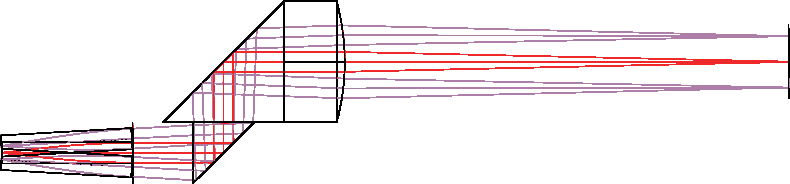
\includegraphics[width=10cm]{figures/30_DesignSimulation/Optical/beamsplitter.pdf}
      \caption{ZEMAX schematic of the OCT beampath for the center (red) and marginal (purple) rays.}
      \label{fig:BS}
\end{figure}

\begin{figure}[h!]\centering
      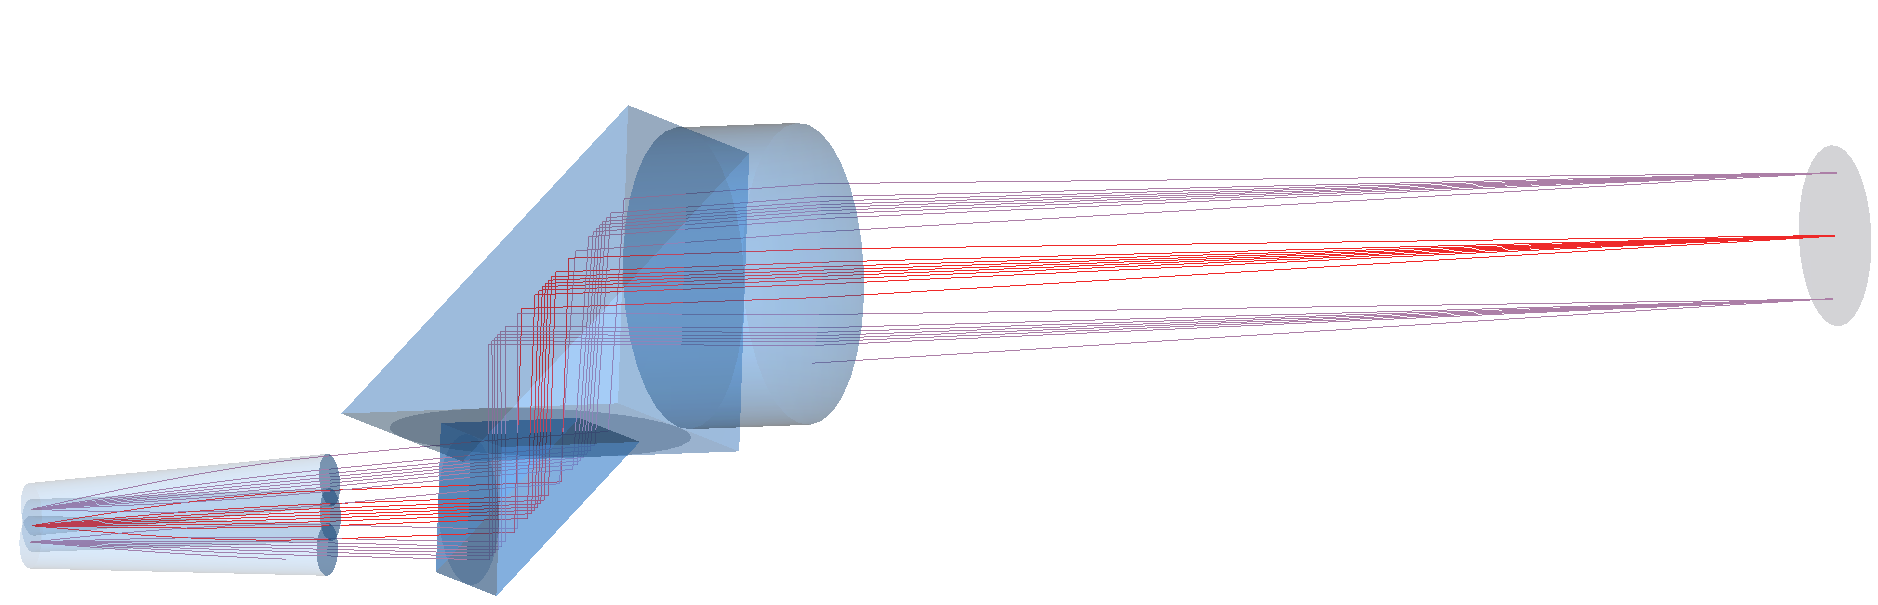
\includegraphics[width=10cm]{figures/30_DesignSimulation/Optical/beamsplitter3D.png}
      \caption{ZEMAX schematic of the OCT beampath for the center (red) and marginal (purple) rays.}
      \label{fig:BS}
\end{figure}

The three overlapping rectangles on the left simulate the rest position (red) and maximum deflection (purple) of the GRIN lens. The gap between GRIN lens and prism is numerically optimized for telecentricity and maximum FOV.

	The low distal-side NA together with the optical quality of the GRIN and spherical lenses enable diffraction limited imaging, as seen in the spot diagrams through focus (Figure \ref{fig:BSspot}) and the MTF curve (Figure \ref{fig:BSMTF}).
	
\begin{figure}[h!]\centering
      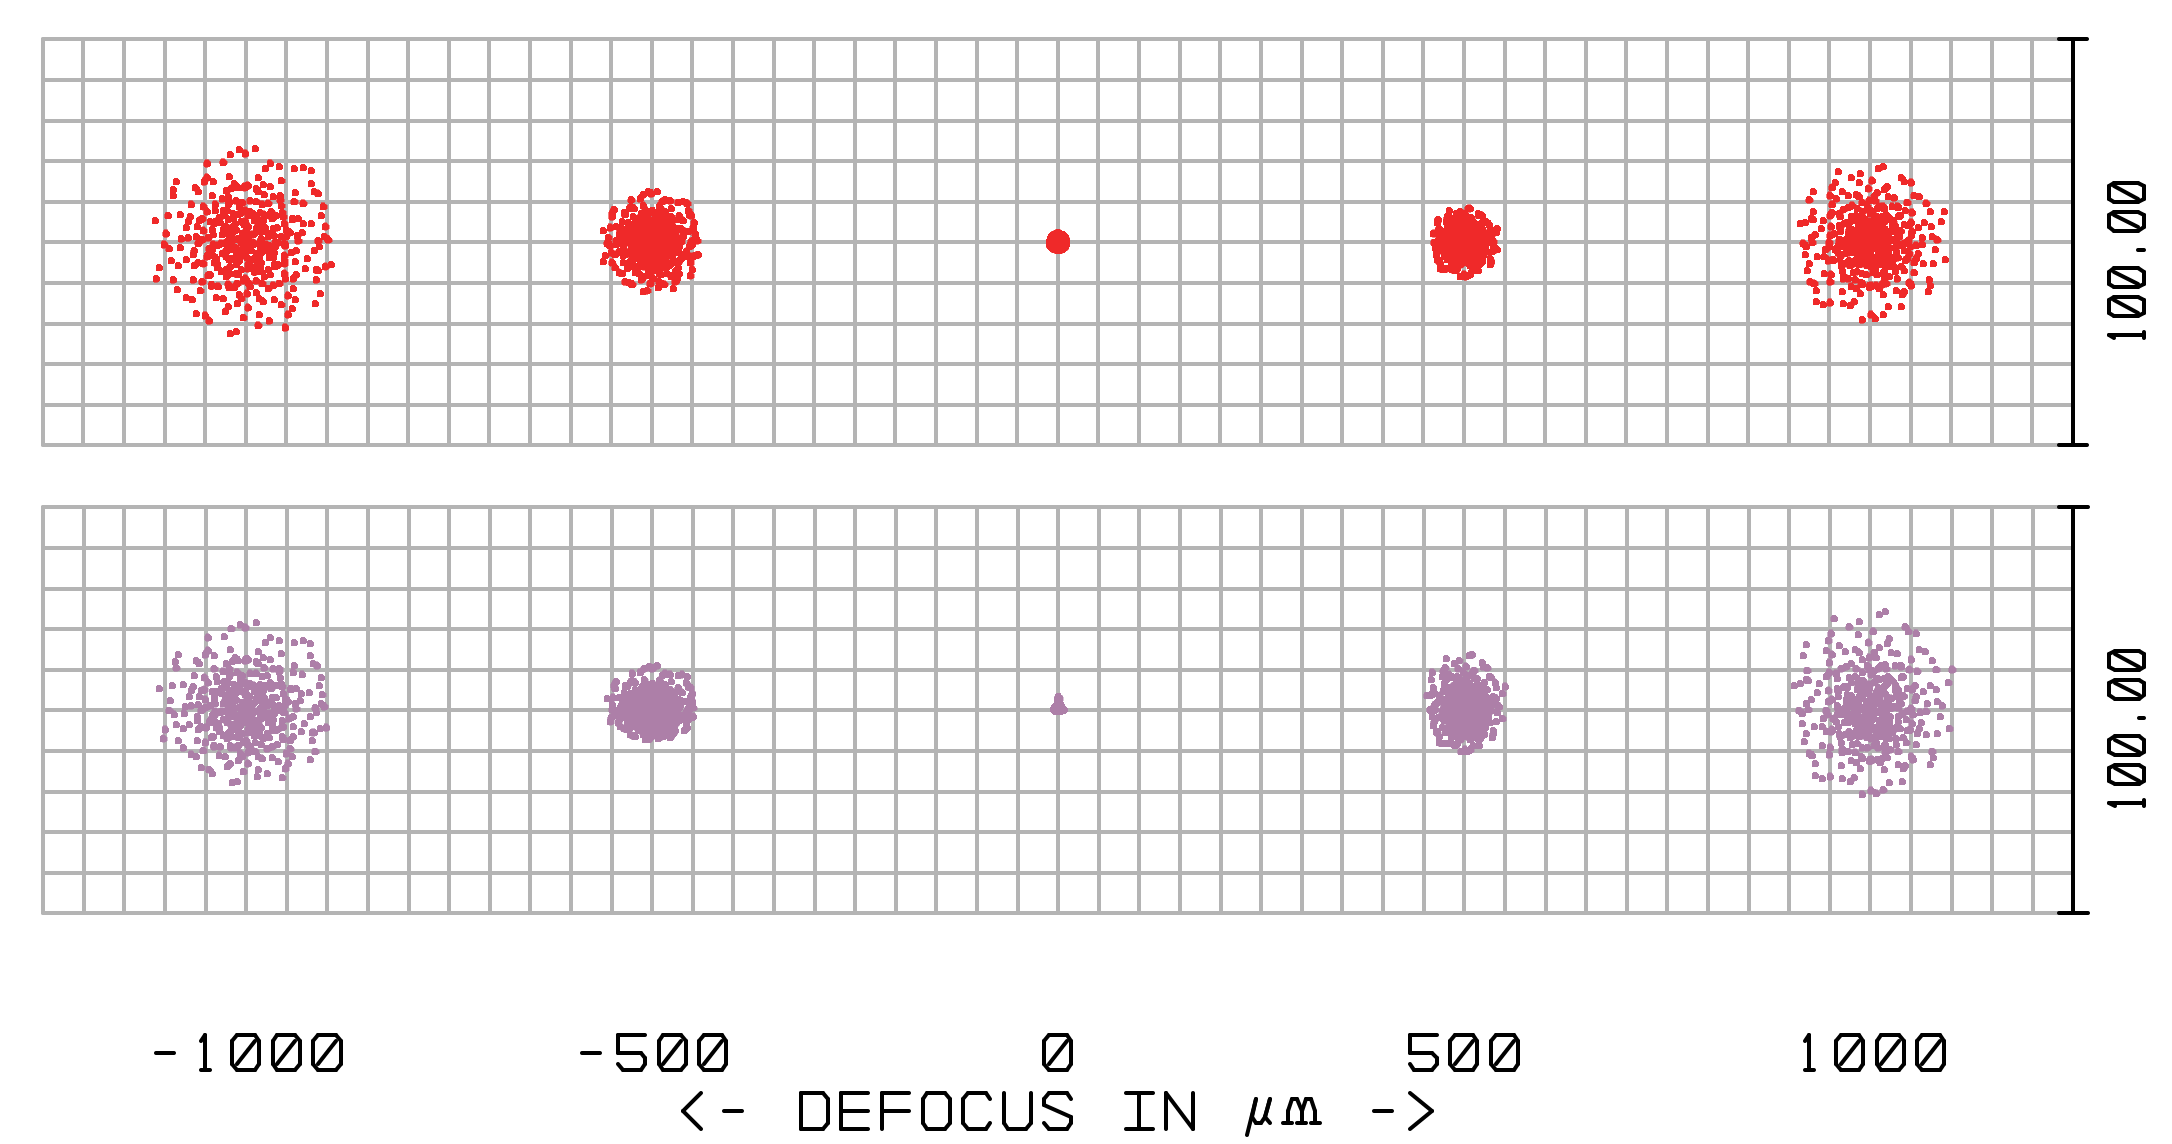
\includegraphics{figures/30_DesignSimulation/Optical/beamsplitterSpot.png}
      \caption{Spot diagram through focus for center (red) and marginal (purple) rays. Dimensions in \SI{}{\micro\meter}.}
      \label{fig:BSspot}
\end{figure}

\begin{figure}[h!]\centering
      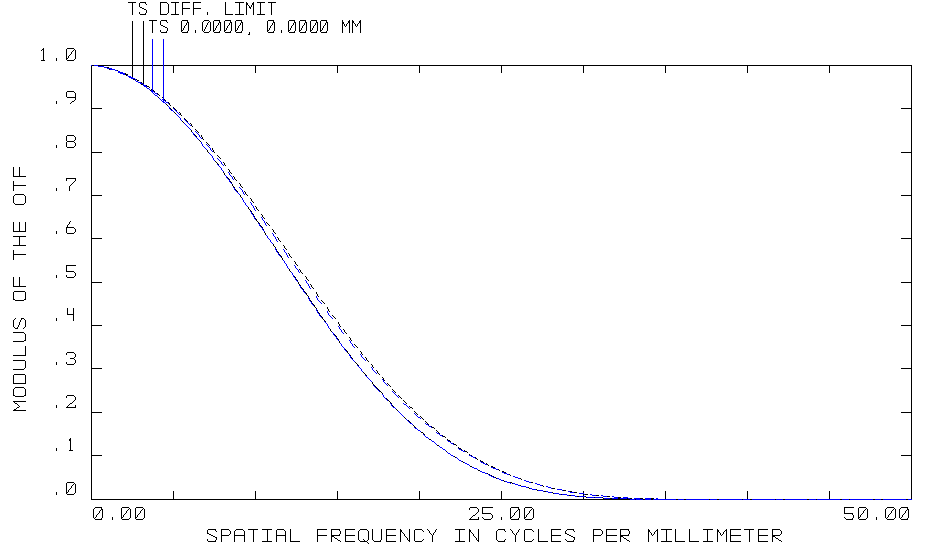
\includegraphics[width=10cm]{figures/30_DesignSimulation/Optical/beamsplitterMTF.png}
      \caption{MTF}
      \label{fig:BSMTF}
\end{figure}

\begin{table}\centering
	\begin{tabular}{rl}\\
		\hline
		\textbf{Distal Side NA} & 0.022 \\ 
		\textbf{Working Distance} & \SI{7.3}{\milli\meter} \\ 
		\textbf{Field of View} & \SI{1.2}{\milli\meter} \\ 
		\textbf{Depth of Field} & \SI{3.4}{\milli\meter} \\ 
		\textbf{Lateral Resolution} & \SI{43}{\micro\meter} \\ 
		\hline
	\end{tabular} 
    \caption{Simulated optical performance and characteristics of OCT modality. All resolution values follow the Rayleigh convention.}
    \label{tab:simRes}
\end{table}


\subsubsection{Minimization of backreflections}
In Fourier Domain OCT, any backreflection coming from the probe increases the background intensity and therefore reduces the penetration depth and contrast of the resultant image. Thus every source of backreflection in the design is carefully considered and reduced:

\paragraph{Fiber-GRIN Interface}
Starting from the proximal side, the fiber-GRIN interface consists of two parallel glass surfaces separated by a small gap. Although the beam is not collimated in this region, a small portion of light can be coupled back to the fiber. In order to minimize any backreflections, they are glued using a refractive-index-matched optical adhesive (\textit{NOA 76}, from \textit{Norland Products}). Thus, the maximum refractive index step is reduced to \SI{0.05}{}.
%Fiber 1.45670,NOA 1.51,GRIN 1.515 -> 275 ppm

\paragraph{GRIN-Air Interface} The next interface is the distal facet of the GRIN lens. This is the most critical interface: Regardless of the scanning angle, it exhibits normal, collimated light incidence. To avoid this problem without resorting to delicate and expensive antireflection coatings (ARC), the GRIN lenses are manufactured with a \SI{1}{\degree} tilted exit facet. According to geometrical optics, this tilt induces a vertical shift in the position of the backreflected focal point, according to equation \ref{eq:tilt}:

\begin{equation}
\Delta y = f \tan(2\alpha) = \SI{0.91}{\milli\meter} \cdot \tan (\SI{2}{\degree}) = \SI{31}{\micro\meter}
\label{eq:tilt}
\end{equation}

The result is visible in the simulation from Figure \ref{fig:tilt}: the backreflected light is focused back with a \SI{31}{\micro\meter} offset, therefore missing the core of the fiber -- which has a diameter inferior to \SI{5}{\micro\meter}.

\begin{figure}[h!]\centering
      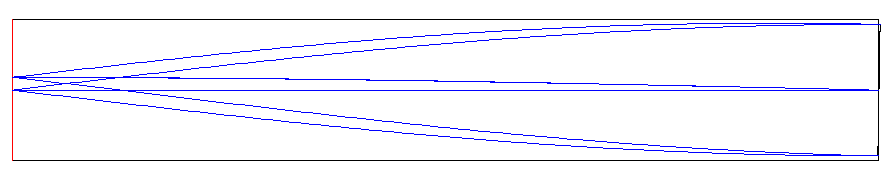
\includegraphics[width=10cm]{figures/30_DesignSimulation/Optical/backreflection.png}
      \caption{Simulation of backreflected light upon the distal end of a GRIN lens with a \SI{1}{\degree} tilted facet.}
      \label{fig:tilt}
\end{figure}

\paragraph{Air-Prism Interface} Due to collimated incidence, this interface exhibits can produce backreflections, but only in a single position of the GRIN lens -- where both facets are parallel. An ARC would be nevertheless beneficial. 

\paragraph{Objective Lens - Air Interface} After the prism, the beamsplitter and objective lens are cemented together, making any backreflections negligible. The objective lens has an interface with air, but due to the curved surface, the light won't be coupled back in a significantly. Nevertheless, the distal surface of the lens are ARC.

%%*****************************************************************************
\newpage
\subsection{Mechanical Design}
%%*****************************************************************************

The fiber scanner uses resonance to amplify the tiny movement of the piezo tube into an angular deflection of the GRIN lens. Therefore, its geometrical and mechanical characteristics fully define the operating frequency range, and with it, the optical sampling.

\begin{figure}[h!]\centering
      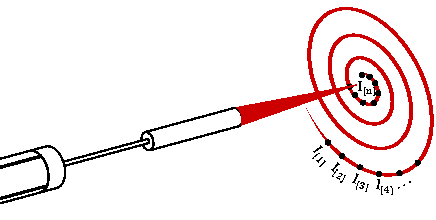
\includegraphics[width=10cm]{figures/30_DesignSimulation/Mechanical/spiralScanning.pdf}
      \caption{Movement of the laser spot through time (red) and acquired points (black)}
      \label{fig:spiralScanning}
\end{figure}

The number of sample points $N_{ring}$ that can be acquired in ring depend on the resonant frequency of the scanner and the sampling frequency of the OCT system:

\begin{equation}
N_{ring} = \frac{f_{sampling}}{f_{resonance}}
\label{eq:nring}
\end{equation}

As OCT systems have a relatively small sampling frequency (\SI{100}{\kilo\hertz}), we need to decrease the resonant frequency below \SI{1}{kHz} to achieve more than 100 points per ring. The following paragraphs describe how to reduce this frequency:

\subsubsection{Resonant frequency calculation}
Following Euler Bernoulli theory, the spring constant for a fixed-free, point loaded cantilever is given by Equation \ref{eq:EB}: 

\begin{equation}
K_{cantilever} = \frac{3 E I}{L^3} = \frac{3 \pi}{4} \frac{E r^4}{L^3}
\label{eq:EB}
\end{equation}
\noindent
considering that the moment of inertia of the cylindrical fiber is given by $I_{fiber} = \frac{\pi}{4} r^4$.

Approximating the fiber - GRIN assembly as a weightless, flexible, fixed-free cantilever and concentrating the weight of the GRIN lens in its center of gravity, we can estimate its resonant frequency by applying the ideal mass-spring harmonic resonator equation for the first resonant mode (Eq. \ref{eq:fres}) \footnote{In order to assess the error of this approximation, we repeated the calculation of the resonant frequency using the method described in \cite{Huo2010}. In the plotted range, the error was smaller than 2\%.}. 

\begin{equation}
f_{res} = \frac{1}{2 \pi} \sqrt{\frac{K_{cantilever}}{m_{\mathit{GRIN}}}} 
\label{eq:fres}
\end{equation}

As we can observe from equation \ref{eq:EB} and \ref{eq:fres}, the resonance frequency increases quadratically with the diameter of the fiber. Therefore, by choosing a fiber with \SI{80}{\micro\meter} instead of the standard \SI{125}{\micro\meter}, the resonance frequency can be lowered from \SI{1900}{\hertz} to \SI{770}{\hertz} for a \SI{4.5}{\milli\meter} scanner.

The resonant frequency of a cantilever formed by a \SI{80}{\micro\meter} fused silica with the chosen GRIN lens is computed in Figure \ref{fig:freq}.

\begin{figure}[h!]\centering
      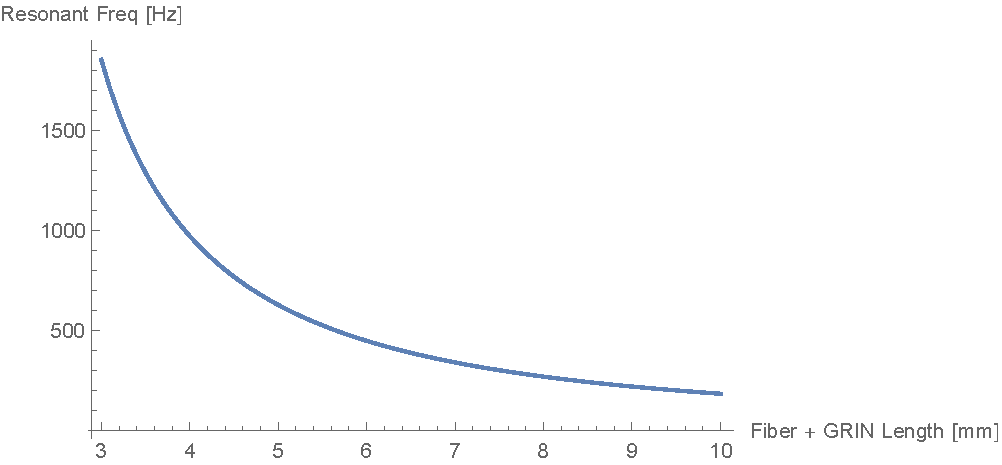
\includegraphics[width=10cm]{figures/30_DesignSimulation/Mechanical/fres.pdf}
      \caption{Resonant frequency as a function of the scanning tip length (fiber + GRIN lens).}
      \label{fig:freq}
\end{figure}

\subsubsection{COMSOL simulation}
In order to validate the theoretical analysis of the previous section, we performed a multiphysics FEM analysis using COMSOL. For that matter, the piezoactuator was modeled as a radially polarized linear piezoelectric material and the rest of the structure as elastic material. The input voltage is added as an harmoniacally excitated symmetrical potential between the top and bottom electrodes of the tube and then an AC simulation was performed. 

As the system undergoes small deflections, it is simulated assuming linear behavior \cite{Fertis2006}.

Note that, as the system is working at its resonance, it is very difficult to simulate the oscillation amplitude, as it depends on its damping factor, which should be obtained experimentally. Figure \ref{fig:defle} shows the AC simulation of the scanner.

\begin{figure}[h!]\centering
      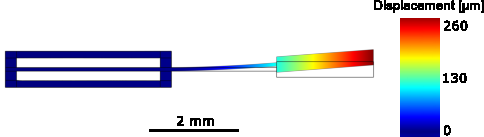
\includegraphics[width=10 cm]{figures/30_DesignSimulation/Mechanical/deflection.pdf}
      \caption{COMSOL simulation of the total deflection in \SI{}{\micro\meter}  at resonance (\SI{762}{\hertz}).}
      \label{fig:defle}
\end{figure}

\begin{figure}[h!]\centering
      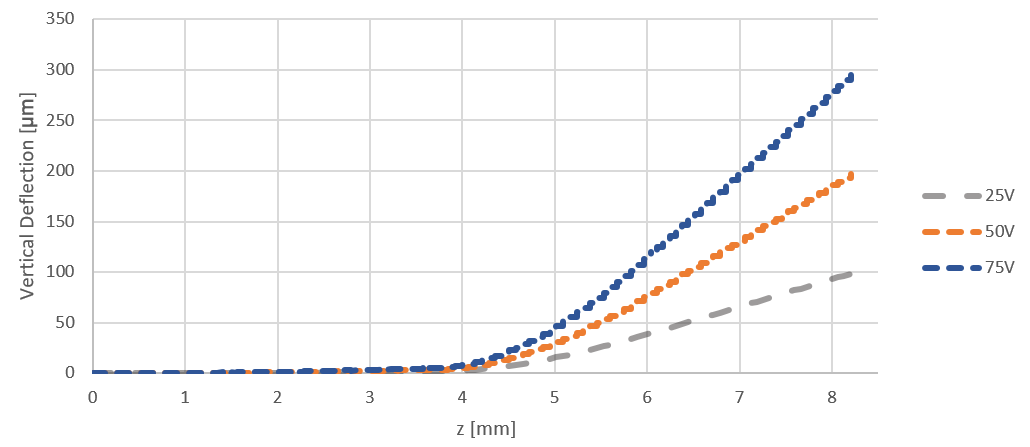
\includegraphics[width=10 cm]{figures/30_DesignSimulation/Mechanical/vsweep.png}
      \caption{Bending line of the resonant tip (fiber + GRIN) VS voltage}
      \label{fig:vsweep}
\end{figure}

\begin{figure}[h!]\centering
      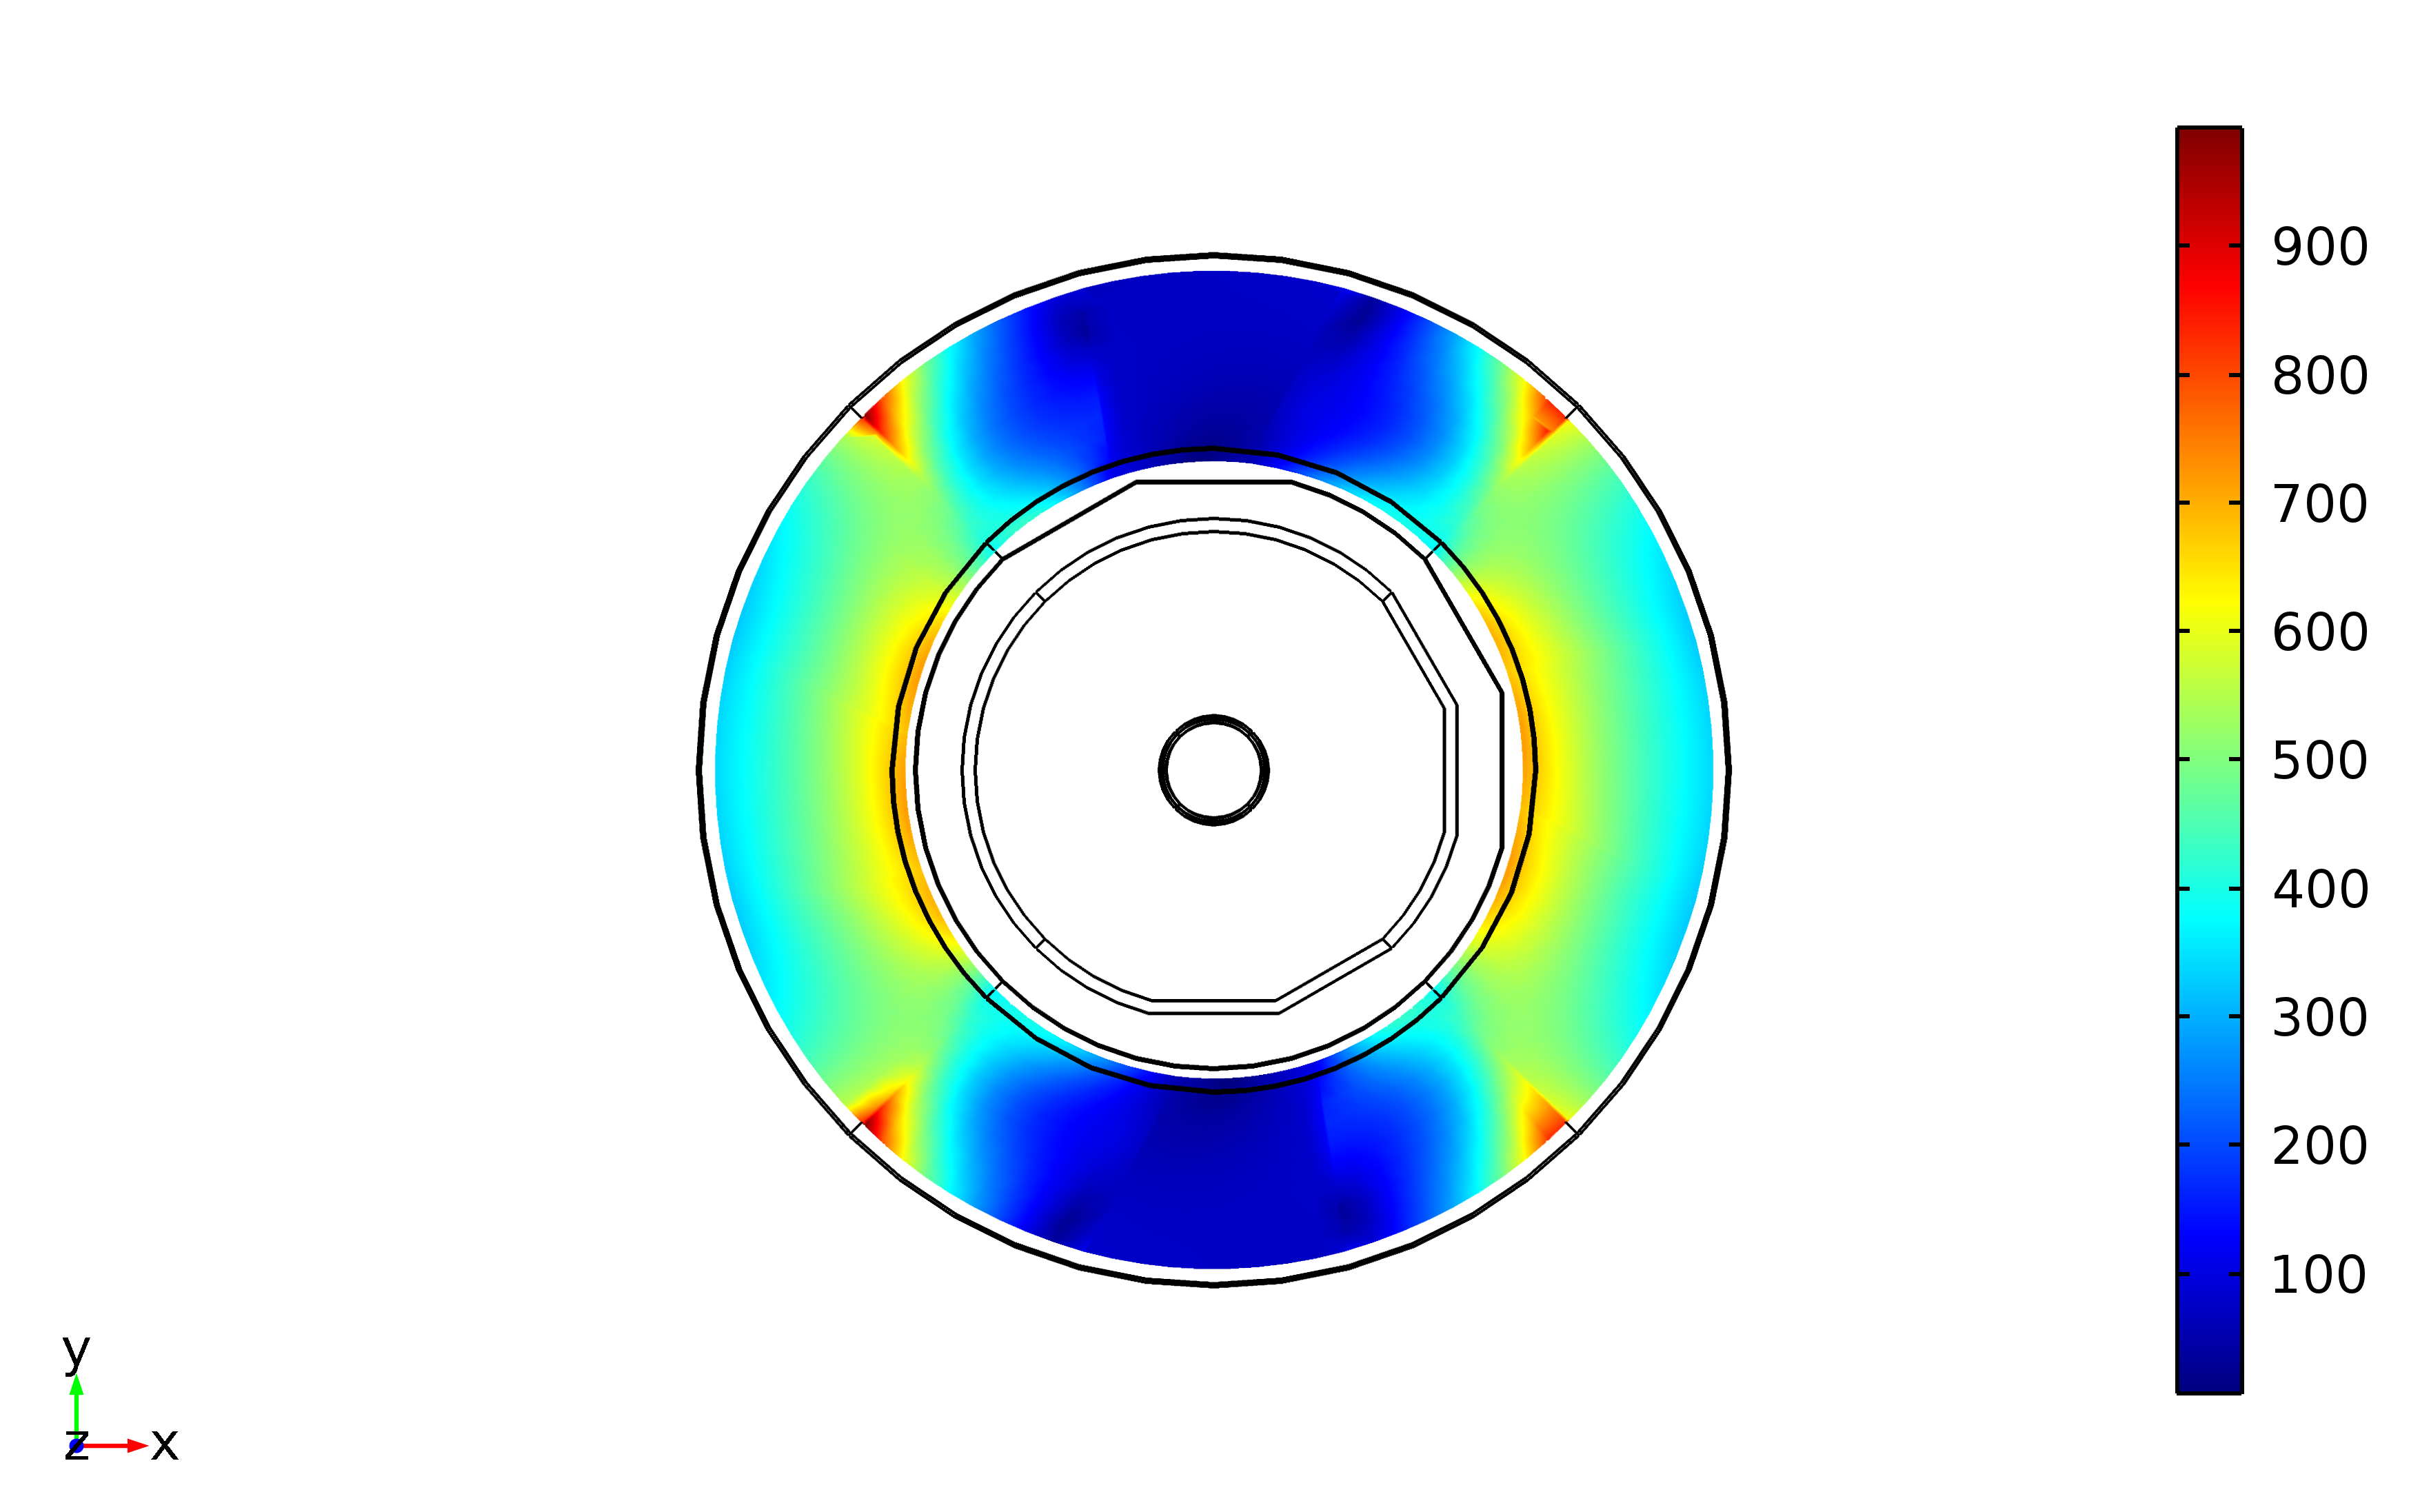
\includegraphics[width=10 cm]{figures/30_DesignSimulation/Mechanical/field.png}
      \caption{Magnitude of the electrical field [\SI{}{\kilo \volt / \meter}] inside a cross-section of the piezotube with an excitation voltage of $\pm \SI{75}{\volt}$}.
      \label{fig:field}
\end{figure}


%%*****************************************************************************
\newpage
\subsection{Overview of the implemented Design}
%%*****************************************************************************
\begin{figure}[h!]\centering 
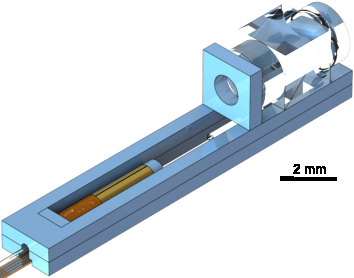
\includegraphics[width=10cm]{figures/30_DesignSimulation/Overview/BimodalBenchDoubleLens.pdf}
      \caption{Bimodal Probe CAD render with annotations}
      %\label{}
\end{figure}


